\begin{figure*}[ht!]
    \centering
    \includegraphics[width=0.95\textwidth]{img/network/LF-SATNet.pdf}
    % \tabcolsep=0.04cm
    % \renewcommand{\arraystretch}{0.8}
    % \begin{tabular}{cc}
    %     \multicolumn{2}{c}{\includegraphics[width=0.4\textwidth]{img/network/LF-SATNet.pdf}} \\
    %     \includegraphics[height=0.09\textwidth]{img/network/SATrans.pdf} &
    %     \includegraphics[height=0.09\textwidth]{img/network/ATrans.pdf} \\
    % \end{tabular} \\
    \vspace{-6pt}
    \caption{Illustration of M2MT-Net and its components. (a) depicts the overview of M2MT. (b) and (c) illustrate the details of a M2MT Transformer and an angular Transformer. These two components constitute a Correlation Block in (d).} \label{fig:M2MT}
\end{figure*}
    

\section{Methodology}
\subsection{Problem Formulation} \label{section:Preliminary}
In formal terms, the procedure of LFSR is to upsample the spatial resolution from a low-resolution (LR) LF image $I_{LR}$ to a super-resolved (SR) LF image $I_{SR}$, which serves as an approximation to the corresponding high-resolution (HR) LF image $I_{HR}$. It can be denoted as
\begin{equation}\label{eq:obj}
\begin{split}
    I_{SR} = \mathcal{F}(I_{LR}), & \quad I_{LR}(u,v,x,y) \in \mathbb{R}^{U \times V \times W \times H \times C}, \\
    & \quad I_{SR}(u,v,x,y) \in \mathbb{R}^{U \times V \times rW \times rH \times C}
\end{split}
\end{equation}
where $(U, V)$ and $(W, H)$ stand for the LR image's angular and spatial resolutions respectively, $C$ denotes the channel dimension, $(u, v)$ indicates an angular location, $(x, y)$ indicates a spatial location, while $r$ represents the scale factor. 

A LF image or tensor, as shown in Figure \ref{fig:Cubes}(a), can be reshaped into various forms to reveal distinctive subspaces. These encompass a spatial tensor $I_S$, revealing the spatial subspace $(W, H)$ depicted in Figure \ref{fig:Cubes}(b), an angular tensor $I_A$ in the angular subspace $(U, V)$ depicted in Figure \ref{fig:Cubes}(c), and EPI tensors $I_{EPI-i}$ which expose the EPI subspace consisting of a spatial and an angular dimension. Figure \ref{fig:Cubes}(d) illustrates $(U, W)$, a variant of EPI tensor.

\subsection{Network Architecture}
The architecture of our proposed M2MT-Net is depicted in Figure \ref{fig:M2MT}(a). It adopts a streamlined yet effective design, comprising three phases. The initial phase involves preliminary feature extraction, accomplished through $n_1$ spatial convolutions. The crux of our architecture, the second component, encompasses a sequence of $n_2$ correlation blocks. Each block incorporates two distinctive Transformers, namely a Many-to-Many Transformer (M2MT) and an angular Transformer, operating consecutively. A simplified visualization of a correlation block is given in Figure \ref{fig:M2MT}(d). The last phase is pixel generation, which upsamples the extracted features by expanding the channel dimensions by $r^2$ times with a $1 \times 1$ convolution, followed by a pixel shuffler to increase the spatial resolution from $U \times V \times W \times H \times (C \times r^2)$ to $U \times V \times rW \times rH \times C$, and lastly, a $3 \times 3$ convolution to squeeze the channels. Additionally, residual learning is enforced to allow the network to effectively capture residual information by learning from the differences between the HR and the bicubic-interpolated LR input. Also, within each correlation block, a residual skip connection is utilized to improve the information flow.

\subsection{Many-to-Many Transformer}
As the pivotal component, M2MT is proposed to mitigate the challenge posed by subspace isolation. Its objective is to holistically extract spatial-angular features with all spatial and angular cues from a LF image.

A simplified illustration of M2MT is depicted in Figure \ref{fig:M2MT} (b), and a detailed one in Figure \ref{fig:Cubes} (e). Specifically, given a 4D LF tensor in a batch $I \in \mathbb{R}^{B \times U \times V \times W \times H \times C}$, it initiates by reshaping it into a spatial tensor $I_{\tilde{S}}$ in a special form. Diverging from the conventional approach of merging angular dimensions with the batch dimension as shown in Figure \ref{fig:Cubes}(b), which yields a spatial tensor $I_{S}$ of dimensions $(BUV \times WH \times C)$ with $WH$ as tokens and $C$ as embedding, we instead merge the angular dimensions with the channel dimensions, resulting in a shape of $(B \times WH \times UVC)$. This approach prepares the tensor for the following correlation encoding process, transforming it into a correlation tensor denoted as $I_{Cor}$ using a linear layer:

\begin{equation}
I_{Cor} = L_{encode}(I_{\tilde{S}}), \quad I_{Cor} \in \mathbb{R}^{B \times WH \times C_{Cor}}
\end{equation}
where $L_{encode}$ represents a linear layer with a projection matrix $W_{encode} \in \mathbb{R}^{UVC \times C_{Cor}}$. The resultant $I_{Cor}$ aggregates the angular correlations at each spatial location. This schema facilitates the succeeding Transformer to invoke the self-attention mechanism in the spatial subspace while concurrently tapping into correlation information from all SAIs. The self-attention mechanism is formally defined as
\begin{equation}
    \begin{aligned}
        \label{eq:self-attention}
        \hat{I}_{Cor} & = \text{Self-Attention}(Q, K, V) \\
                     & = \text{softmax}\left(\frac{QK^T}{\sqrt{d_k}}\right), \\
               Q,K,V & = L_Q({I_{Cor}}),L_K({I_{Cor}}),L_V({I_{Cor}})
    \end{aligned}
\end{equation}

In this context, $\hat{I}_{Cor}$ signifies the tensor enhanced by self-attention. $L_Q$, $L_K$, and $L_V$ are the linear layers for calculating queries, keys, and values respectively. Notably, we replace commonly used predefined positional encodings with two $3 \times 3$ spatial convolutions to capture locality as suggested by \cite{chuCPVT_arxiv2021}.

As last, a linear layer is employed to decode $\hat{I}_{Cor}$ and recover the angular dimensions, resulting in the output feature tensor $\hat{I}$:
\begin{equation}
    \hat{I} = L_{decode}(\hat{I}_{Cor})
\end{equation}

In essence, M2MT fulfills the objectives of Equation \ref{eq:after}, where $I_{Cor}$ aggregates all SAI information at each spatial location:
\begin{equation}
    I_{Cor}(x, y) \simeq \{I(\bar{u}, \bar{v}, x, y)\}_{(\bar{u}, \bar{v}) \in \mathbb{R}^{U \times V}},
\end{equation}
and the self-attention mechanism models the long-range dependencies among the spatial locations:
\begin{equation}
    \hat{I}_{Cor}(x, y) \simeq \{I(u, v, \bar{x}, \bar{y})\}_{(\bar{x}, \bar{y}) \in \mathbb{R}^{W \times H}} \\
\end{equation}

Consequently, M2MT is enabled to access the entirety of LF data in a non-local context spatially and angularly with no information remain isolated within the batch dimension:
\begin{equation}
    \hat{I}(u, v, x, y) \simeq \{I(\bar{u}, \bar{v}, \bar{x}, \bar{y})\}_{(\bar{u}, \bar{v}, \bar{x}, \bar{y}) \in \mathbb{R}^{U \times V \times W \times H}}
\end{equation}
where the inference process for any given location $(u, v, x, y)$ is many-to-one. Since M2MT concurrently infers all pixels, the overall operation is inherently many-to-many.

\begin{table*}[t!]
    \caption{Quantitative comparisons with the state-of-art methods at $2 \times$ and $4 \times$ scales across various datasets. PSNR / SSIM are used as evaluation metrics. The best and second-best results are in bold and underlined.}
    \label{tab:overall}
    \centering
    \begin{tabular}{|l|c|c|c|c|c|c|c|}
    \hline
    Method & Scale & EPFL & HCInew & HCIold & INRIA & STFgantry \\
    \hline
    LFSSR \cite{yeungSAS_LFSR2019}	            & $2\times$ & 33.67/0.9744                          & 36.80/0.9749                          & 43.81/0.9938                              & 35.28/0.9832                            &	37.94/0.9898                            \\
    LF-ATO \cite{jinLFSSRATO_2020}	            & $2\times$ & 34.27/0.9757                          & 37.24/0.9767                          & 44.21/0.9942                              & 36.17/0.9842                            &	39.64/0.9929                            \\
    LF-InterNet \cite{wangLfInterNet_ECCV2020}	& $2\times$ & 34.11/0.9760                          & 37.17/0.9763                          & 44.57/0.9946                              & 35.83/0.9843                            &	38.44/0.9909                            \\
    LF-IINet \cite{liuLFIINet_TMM2021}	        & $2\times$ & 34.73/0.9773                          & 37.77/0.9790                          & 44.85/0.9948                              & 36.57/0.9853                            &	39.89/0.9936                            \\
    DKNet \cite{huDKNet_TIM2022}                & $2\times$ & 34.01/0.9759                          & 31.36/0.9780                          & 44.19/0.9942                              & 35.80/0.9843                            & 39.59/0.9910                            \\
    DPT	\cite{wangDPT_AAAI2022}                 & $2\times$ & 34.49/0.9758                          & 37.36/0.9771                          & 44.30/0.9943                              & 36.41/0.9843                            &	39.43/0.9926                            \\
    DistgSSR \cite{wangDistgSSR_TIP2022}	    & $2\times$ & 34.81/0.9787                          & 37.96/0.9796                          & 44.94/0.9949                              & 36.59/0.9859                            &	40.40/0.9942                            \\
    LFT \cite{liangLFT_SPL2022}	                & $2\times$ & 34.80/0.9781                          & 37.84/0.9791                          & 44.52/0.9945                              & 36.60/0.9855                            &	40.51/0.9941                            \\
    EPIT \cite{liangEPIT_arXiv2023}	            & $2\times$ & 34.83/0.9775                          & 38.23/\underline{0.9810}              & 45.06/0.9949                              & 36.67/0.9853                            &	\textbf{42.17}/\textbf{0.9957}          \\
    \hline
    M2MT-Net (Ours)                   & $2\times$ & \underline{35.36}/\underline{0.9804}  & \underline{38.29}/0.9806              & \underline{45.14}/\underline{0.9951}      & \underline{36.99}/\underline{0.9867}    & 40.80/0.9947                            \\
    M2MT-Net* (Ours)                  & $2\times$ & \textbf{35.56}/\textbf{0.9812}        & \textbf{38.48}/\textbf{0.9811}        & \textbf{45.39}/\textbf{0.9954}            & \textbf{37.19}/\textbf{0.9870}          & \underline{41.23}/\underline{0.9951}    \\
    \hline\hline    
    LFSSR \cite{yeungSAS_LFSR2019}              & $4\times$ & 28.60/0.9118                          & 30.93/0.9145                          & 36.91/0.9696                              & 30.59/0.9467                              & 30.57/0.9426 \\
    LFSSR-ATO \cite{jinLFSSRATO_2020}           & $4\times$ & 28.51/0.9115                          & 30.88/0.9135                          & 37.00/0.9699                              & 30.71/0.9484                              & 30.61/0.9430 \\
    LF-InterNet \cite{wangLfInterNet_ECCV2020}  & $4\times$ & 28.81/0.9162                          & 30.96/0.9161                          & 37.15/0.9716                              & 30.78/0.9491                              & 30.36/0.9409 \\
    LF-IINet \cite{liuLFIINet_TMM2021}          & $4\times$ & 29.04/0.9188                          & 31.33/0.9208                          & 37.62/0.9734                              & 31.03/0.9515                              & 31.26/0.9502 \\
    DKNet \cite{huDKNet_TIM2022}                & $4\times$ & 28.85/0.9174                          & 31.17/0.9186                          & 37.31/0.9721                              & 30.80/0.9501                              & 30.85/0.9461 \\
    DPT \cite{wangDPT_AAAI2022}                 & $4\times$ & 28.94/0.9170                          & 31.20/0.9188                          & 37.41/0.9721                              & 30.96/0.9503                              & 31.15/0.9488 \\
    DisgSSR \cite{wangDistgSSR_TIP2022}         & $4\times$ & 28.99/0.9195                          & 31.38/0.9217                          & 37.56/0.9732                              & 30.99/0.9519                              & 31.65/0.9535 \\
    LFT \cite{liangLFT_SPL2022}                 & $4\times$ & 29.26/0.9210                          & 31.46/0.9218                          & 37.63/0.9735                              & 31.21/0.9524                              & 31.86/0.9548 \\
    EPIT \cite{liangEPIT_arXiv2023}             & $4\times$ & 29.34/0.9197                          & 31.51/0.9231                          & 37.68/0.9737                              & 31.37/0.9526                              & \underline{32.18}/\underline{0.9571} \\
    \hline
    M2MT-Net (Ours)                   & $4\times$ & \underline{29.80}/\underline{0.9277}  & \underline{31.70}/\underline{0.9252}  & \underline{37.99}/\underline{0.9750}      & \underline{31.73}/\underline{0.9556}      & 32.02/0.9560 \\
    M2MT-Net* (Ours)                  & $4\times$ & \textbf{29.94}/\textbf{0.9298}        & \textbf{31.90}/\textbf{0.9272}        & \textbf{38.20}/\textbf{0.9750}            & \textbf{31.89}/\textbf{0.9570}            & \textbf{32.34}/\textbf{0.9587} \\
    \hline
    \multicolumn{6}{l}{\scriptsize * Geometric self-ensemble strategy is applied.}
    \end{tabular}
    % LFSSR-SAV & $4\times$ & 29.37/0.9223 & 31.45/0.9217 & 37.50/0.9721 & 31.27/0.9531 & 31.36/0.9505 \\
    % HLFSR-SSR \cite{hlfsr-ssr}& 29.196/0.9222 & 31.571/\textbf{0.9238} & 37.776/0.9742 & 31.241/\textbf{0.9534} & 31.641/0.9537 \\
    % LF-DET \cite{lfdet}& 29.473/\textbf{0.9230} & 31.558/0.9235 & \textbf{37.843}/\textbf{0.9744} & 31.389/\textbf{0.9534} & 32.139/0.9573 \\
\end{table*}
\begin{figure*}[ht!]
    \centering
    \tabcolsep=0.05cm
    \renewcommand{\arraystretch}{1.0}
    \resizebox{0.98\textwidth}{!}{
    \begin{tabular}{cccccc}
        % Title
        HR &
        IINet &
        DistgSSR &
        LFT &
        EPIT &
        M2MT-Net \\
        \hline
        \vspace{-7pt}
        \\
        % Perforated_Metal_3
        % main image
        \includegraphics[width=0.180\textwidth, height=0.136\textwidth]{img/qual/Perforated_Metal_3/HR-view.annotated.png} &
        \includegraphics[width=0.180\textwidth, height=0.136\textwidth]{img/qual/Perforated_Metal_3/IINet/2_2.png} &
        \includegraphics[width=0.180\textwidth, height=0.136\textwidth]{img/qual/Perforated_Metal_3/DistgSSR/2_2.png} &
        \includegraphics[width=0.180\textwidth, height=0.136\textwidth]{img/qual/Perforated_Metal_3/LFT/2_2.png} &
        \includegraphics[width=0.180\textwidth, height=0.136\textwidth]{img/qual/Perforated_Metal_3/EPIT/2_2.png} &
        \includegraphics[width=0.180\textwidth, height=0.136\textwidth]{img/qual/Perforated_Metal_3/SAT/2_2.png} \\
        % Two images
        \begin{minipage}{0.180\textwidth}
            \centering
            \includegraphics[width=0.46\textwidth, height=0.46\textwidth,cfbox=blue 1pt 0pt]{img/qual/Perforated_Metal_3/HR.annotated.png}
            \includegraphics[width=0.46\textwidth, height=0.46\textwidth,cfbox=red 1pt 0pt]{img/qual/Perforated_Metal_3/HR.LAM.png}
        \end{minipage} &
        \begin{minipage}{0.180\textwidth}
            \centering
            \includegraphics[width=0.46\textwidth, height=0.46\textwidth,cfbox=blue 1pt 0pt]{img/qual/Perforated_Metal_3/IINet/SR.png}
            \includegraphics[width=0.46\textwidth, height=0.46\textwidth,cfbox=red 1pt 0pt]{img/qual/Perforated_Metal_3/IINet/SR.LAM.png}
        \end{minipage} &
        \begin{minipage}{0.180\textwidth}
            \centering
            \includegraphics[width=0.46\textwidth, height=0.46\textwidth,cfbox=blue 1pt 0pt]{img/qual/Perforated_Metal_3/DistgSSR/SR.png}
            \includegraphics[width=0.46\textwidth, height=0.46\textwidth,cfbox=red 1pt 0pt]{img/qual/Perforated_Metal_3/DistgSSR/SR.LAM.png}
        \end{minipage} &
        \begin{minipage}{0.180\textwidth}
            \centering
            \includegraphics[width=0.46\textwidth, height=0.46\textwidth,cfbox=blue 1pt 0pt]{img/qual/Perforated_Metal_3/LFT/SR.png}
            \includegraphics[width=0.46\textwidth, height=0.46\textwidth,cfbox=red 1pt 0pt]{img/qual/Perforated_Metal_3/LFT/SR.LAM.png}
        \end{minipage} &
        \begin{minipage}{0.180\textwidth}
            \centering
            \includegraphics[width=0.46\textwidth, height=0.46\textwidth,cfbox=blue 1pt 0pt]{img/qual/Perforated_Metal_3/EPIT/SR.png}
            \includegraphics[width=0.46\textwidth, height=0.46\textwidth,cfbox=red 1pt 0pt]{img/qual/Perforated_Metal_3/EPIT/SR.LAM.png}
        \end{minipage} &
        \begin{minipage}{0.180\textwidth}
            \centering
            \includegraphics[width=0.46\textwidth, height=0.46\textwidth,cfbox=blue 1pt 0pt]{img/qual/Perforated_Metal_3/SAT/SR.png}
            \includegraphics[width=0.46\textwidth, height=0.46\textwidth,cfbox=red 1pt 0pt]{img/qual/Perforated_Metal_3/SAT/SR.LAM.png}
        \end{minipage} \\
        % PSNR/SSIM
        (a) \textit{Perforated\_Metal\_3} &
        20.95/0.7054 &
        20.64/0.7044 &
        \underline{21.13}/\underline{0.7190} &
        18.76/0.5257 &
        \textbf{22.71}/\textbf{0.8180} \\
        \vspace{-10pt}
        \\
        % LAM
        \raisebox{1.8\height}{
        \resizebox{0.06\textwidth}{!}{
            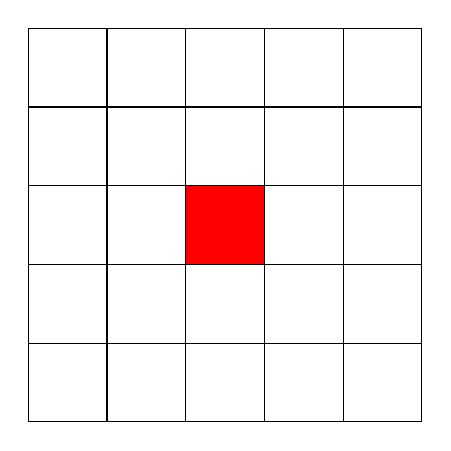
\begin{tikzpicture}
                \foreach \x in {0,1,2,3,4} {
                    \foreach \y in {0,1,2,3,4} {
                        \draw[black, thin] (\x,\y) rectangle (\x+1,\y+1);
                    }
                }
                \fill[red] (2,2) rectangle (3,3);
            \end{tikzpicture}
        } } &
        \imageWithGrid{img/qual/Perforated_Metal_3/IINet/LAM.overlay.png}{0.178\textwidth}{0.178\textwidth} &
        \imageWithGrid{img/qual/Perforated_Metal_3/DistgSSR/LAM.overlay.png}{0.178\textwidth}{0.178\textwidth} &
        \imageWithGrid{img/qual/Perforated_Metal_3/LFT/LAM.overlay.png}{0.178\textwidth}{0.178\textwidth} &
        \imageWithGrid{img/qual/Perforated_Metal_3/EPIT/LAM.overlay.png}{0.178\textwidth}{0.178\textwidth} &
        \imageWithGrid{img/qual/Perforated_Metal_3/SAT/LAM.overlay.png}{0.178\textwidth}{0.178\textwidth} \\
        % DI
        &
        DI = 9.8521 &
        DI = 9.6033 &
        DI = 7.7526 &
        DI = 5.9518 &
        DI = 27.2578 \\\hline

        \vspace{-7pt}
        \\

        % Palais_du_Luxembourg
        % Title
        % HR &
        % IINet &
        % DistgSSR &
        % LFT &
        % EPIT &
        % M2MT \\
        % main image
        \includegraphics[width=0.180\textwidth, height=0.136\textwidth]{img/qual/Palais_du_Luxembourg/HR-view.annotated.png} &
        \includegraphics[width=0.180\textwidth, height=0.136\textwidth]{img/qual/Palais_du_Luxembourg/IINet/1_3.png} &
        \includegraphics[width=0.180\textwidth, height=0.136\textwidth]{img/qual/Palais_du_Luxembourg/DistgSSR/1_3.png} &
        \includegraphics[width=0.180\textwidth, height=0.136\textwidth]{img/qual/Palais_du_Luxembourg/LFT/1_3.png} &
        \includegraphics[width=0.180\textwidth, height=0.136\textwidth]{img/qual/Palais_du_Luxembourg/EPIT/1_3.png} &
        \includegraphics[width=0.180\textwidth, height=0.136\textwidth]{img/qual/Palais_du_Luxembourg/SAT/1_3.png} \\
        % Two images
        \begin{minipage}{0.180\textwidth}
            \centering
            \includegraphics[width=0.46\textwidth, height=0.46\textwidth,cfbox=blue 1pt 0pt]{img/qual/Palais_du_Luxembourg/HR.annotated.png}
            \includegraphics[width=0.46\textwidth, height=0.46\textwidth,cfbox=red 1pt 0pt]{img/qual/Palais_du_Luxembourg/HR.LAM.png}
        \end{minipage} &
        \begin{minipage}{0.180\textwidth}
            \centering
            \includegraphics[width=0.46\textwidth, height=0.46\textwidth,cfbox=blue 1pt 0pt]{img/qual/Palais_du_Luxembourg/IINet/SR.png}
            \includegraphics[width=0.46\textwidth, height=0.46\textwidth,cfbox=red 1pt 0pt]{img/qual/Palais_du_Luxembourg/IINet/SR.LAM.png}
        \end{minipage} &
        \begin{minipage}{0.180\textwidth}
            \centering
            \includegraphics[width=0.46\textwidth, height=0.46\textwidth,cfbox=blue 1pt 0pt]{img/qual/Palais_du_Luxembourg/DistgSSR/SR.png}
            \includegraphics[width=0.46\textwidth, height=0.46\textwidth,cfbox=red 1pt 0pt]{img/qual/Palais_du_Luxembourg/DistgSSR/SR.LAM.png}
        \end{minipage} &
        \begin{minipage}{0.180\textwidth}
            \centering
            \includegraphics[width=0.46\textwidth, height=0.46\textwidth,cfbox=blue 1pt 0pt]{img/qual/Palais_du_Luxembourg/LFT/SR.png}
            \includegraphics[width=0.46\textwidth, height=0.46\textwidth,cfbox=red 1pt 0pt]{img/qual/Palais_du_Luxembourg/LFT/SR.LAM.png}
        \end{minipage} &
        \begin{minipage}{0.180\textwidth}
            \centering
            \includegraphics[width=0.46\textwidth, height=0.46\textwidth,cfbox=blue 1pt 0pt]{img/qual/Palais_du_Luxembourg/EPIT/SR.png}
            \includegraphics[width=0.46\textwidth, height=0.46\textwidth,cfbox=red 1pt 0pt]{img/qual/Palais_du_Luxembourg/EPIT/SR.LAM.png}
        \end{minipage} &
        \begin{minipage}{0.180\textwidth}
            \centering
            \includegraphics[width=0.46\textwidth, height=0.46\textwidth,cfbox=blue 1pt 0pt]{img/qual/Palais_du_Luxembourg/SAT/SR.png}
            \includegraphics[width=0.46\textwidth, height=0.46\textwidth,cfbox=red 1pt 0pt]{img/qual/Palais_du_Luxembourg/SAT/SR.LAM.png}
        \end{minipage} \\
        % PSNR/SSIM
        (b) \textit{Palais\_du\_Luxembourg} &
        18.86/\underline{0.5653} &
        18.62/0.5367 &
        18.90/0.5443 &
        \underline{18.96}/0.5584 &
        \textbf{19.68}/\textbf{0.6739} \\
        \vspace{-10pt}
        \\
        % LAM
        \raisebox{1.8\height}{
        \resizebox{0.06\textwidth}{!}{
            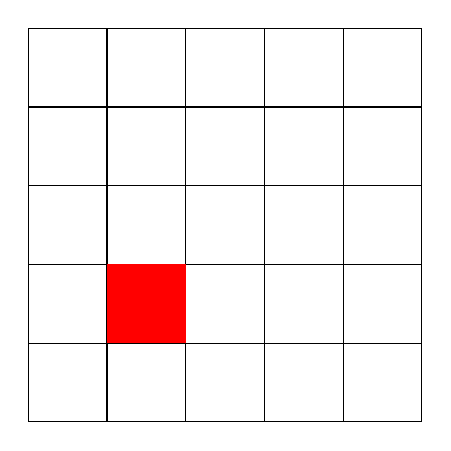
\begin{tikzpicture}
                \foreach \x in {0,1,2,3,4} {
                    \foreach \y in {0,1,2,3,4} {
                        \draw[black, thin] (\x,\y) rectangle (\x+1,\y+1);
                    }
                }
                \fill[red] (1,1) rectangle (2,2);
            \end{tikzpicture}
        } } &
        \imageWithGrid{img/qual/Palais_du_Luxembourg/IINet/LAM.overlay.png}{0.178\textwidth}{0.178\textwidth} &
        \imageWithGrid{img/qual/Palais_du_Luxembourg/DistgSSR/LAM.overlay.png}{0.178\textwidth}{0.178\textwidth} &
        \imageWithGrid{img/qual/Palais_du_Luxembourg/LFT/LAM.overlay.png}{0.178\textwidth}{0.178\textwidth} &
        \imageWithGrid{img/qual/Palais_du_Luxembourg/EPIT/LAM.overlay.png}{0.178\textwidth}{0.178\textwidth} &
        \imageWithGrid{img/qual/Palais_du_Luxembourg/SAT/LAM.overlay.png}{0.178\textwidth}{0.178\textwidth} \\
        % DI
        &
        DI = 8.0609 &
        DI = 7.8105 &
        DI = 4.1552 &
        DI = 6.5223 &
        DI = 21.0431 \\\hline

        \vspace{-7pt}
        \\

        % Bicycle
        % Title
        % HR &
        % IINet &
        % DistgSSR &
        % LFT &
        % EPIT &
        % M2MT \\
        % main image
        \includegraphics[width=0.180\textwidth, height=0.136\textwidth]{img/qual/Bicycle/HR-view.annotated.png} &
        \includegraphics[width=0.180\textwidth, height=0.136\textwidth]{img/qual/Bicycle/IINet/2_2.png} &
        \includegraphics[width=0.180\textwidth, height=0.136\textwidth]{img/qual/Bicycle/DistgSSR/2_2.png} &
        \includegraphics[width=0.180\textwidth, height=0.136\textwidth]{img/qual/Bicycle/LFT/2_2.png} &
        \includegraphics[width=0.180\textwidth, height=0.136\textwidth]{img/qual/Bicycle/EPIT/2_2.png} &
        \includegraphics[width=0.180\textwidth, height=0.136\textwidth]{img/qual/Bicycle/SAT/2_2.png} \\
        % Two images
        \begin{minipage}{0.180\textwidth}
            \centering
            \includegraphics[width=0.46\textwidth, height=0.46\textwidth,cfbox=blue 1pt 0pt]{img/qual/Bicycle/HR.annotated.png}
            \includegraphics[width=0.46\textwidth, height=0.46\textwidth,cfbox=red 1pt 0pt]{img/qual/Bicycle/HR.LAM.png}
        \end{minipage} &
        \begin{minipage}{0.180\textwidth}
            \centering
            \includegraphics[width=0.46\textwidth, height=0.46\textwidth,cfbox=blue 1pt 0pt]{img/qual/Bicycle/IINet/SR.png}
            \includegraphics[width=0.46\textwidth, height=0.46\textwidth,cfbox=red 1pt 0pt]{img/qual/Bicycle/IINet/SR.LAM.png}
        \end{minipage} &
        \begin{minipage}{0.180\textwidth}
            \centering
            \includegraphics[width=0.46\textwidth, height=0.46\textwidth,cfbox=blue 1pt 0pt]{img/qual/Bicycle/DistgSSR/SR.png}
            \includegraphics[width=0.46\textwidth, height=0.46\textwidth,cfbox=red 1pt 0pt]{img/qual/Bicycle/DistgSSR/SR.LAM.png}
        \end{minipage} &
        \begin{minipage}{0.180\textwidth}
            \centering
            \includegraphics[width=0.46\textwidth, height=0.46\textwidth,cfbox=blue 1pt 0pt]{img/qual/Bicycle/LFT/SR.png}
            \includegraphics[width=0.46\textwidth, height=0.46\textwidth,cfbox=red 1pt 0pt]{img/qual/Bicycle/LFT/SR.LAM.png}
        \end{minipage} &
        \begin{minipage}{0.180\textwidth}
            \centering
            \includegraphics[width=0.46\textwidth, height=0.46\textwidth,cfbox=blue 1pt 0pt]{img/qual/Bicycle/EPIT/SR.png}
            \includegraphics[width=0.46\textwidth, height=0.46\textwidth,cfbox=red 1pt 0pt]{img/qual/Bicycle/EPIT/SR.LAM.png}
        \end{minipage} &
        \begin{minipage}{0.180\textwidth}
            \centering
            \includegraphics[width=0.46\textwidth, height=0.46\textwidth,cfbox=blue 1pt 0pt]{img/qual/Bicycle/SAT/SR.png}
            \includegraphics[width=0.46\textwidth, height=0.46\textwidth,cfbox=red 1pt 0pt]{img/qual/Bicycle/SAT/SR.LAM.png}
        \end{minipage} \\
        % PSNR/SSIM
        (c) \textit{Bicycle} &
        27.01/0.8333 &
        26.85/0.8308 &
        27.14/0.8283 &
        \underline{27.21}/\underline{0.8367} &
        \textbf{27.37}/\textbf{0.8390} \\
        \vspace{-10pt}
        \\
        % LAM
        \raisebox{1.8\height}{
        \resizebox{0.06\textwidth}{!}{
            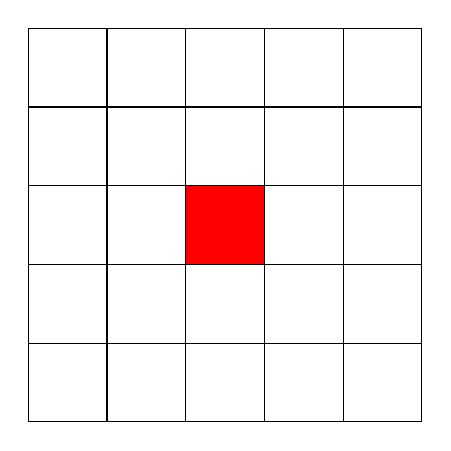
\begin{tikzpicture}
                \foreach \x in {0,1,2,3,4} {
                    \foreach \y in {0,1,2,3,4} {
                        \draw[black, thin] (\x,\y) rectangle (\x+1,\y+1);
                    }
                }
                \fill[red] (2,2) rectangle (3,3);
            \end{tikzpicture}
        } } &
        \imageWithGrid{img/qual/Bicycle/IINet/LAM.overlay.png}{0.178\textwidth}{0.178\textwidth} &
        \imageWithGrid{img/qual/Bicycle/DistgSSR/LAM.overlay.png}{0.178\textwidth}{0.178\textwidth} &
        \imageWithGrid{img/qual/Bicycle/LFT/LAM.overlay.png}{0.178\textwidth}{0.178\textwidth} &
        \imageWithGrid{img/qual/Bicycle/EPIT/LAM.overlay.png}{0.178\textwidth}{0.178\textwidth} &
        \imageWithGrid{img/qual/Bicycle/SAT/LAM.overlay.png}{0.178\textwidth}{0.178\textwidth} \\
        % DI
        &
        DI = 11.2056 &
        DI = 6.4649 &
        DI = 4.3732 &
        DI = 6.5302 &
        DI = 19.2823 \\
    \end{tabular}
    }

    \caption{Visualization of selected samples in the $4\times$ task. In each sample, the following result is provided for each compared method: the SAI, the zoom-in views from the blue and red boxes, the PSNR/SSIM of the red box, the local attribution map (LAM) of the red box and its diffusion index (DI). The best and second-best PSNR/SSIM are in bold and underlined. The angular location indicator is given below the HR.}
    \label{fig:Qual}
\end{figure*}
\begin{figure*}[ht]
    \centering
    \tabcolsep=0.05cm
    \renewcommand{\arraystretch}{1.0}
    \begin{tabular}{c}
        \includegraphics[width=0.98\textwidth]{img/qual_matrix/Perforated_Metal_3.h5.pdf} \\
        (a) \textit{Perforated\_Metal\_3} \\
        \includegraphics[width=0.98\textwidth]{img/qual_matrix/Palais_du_Luxembourg.h5.pdf} \\
        (b) \textit{Palais\_du\_Luxembourg} \\
        \includegraphics[width=0.98\textwidth]{img/qual_matrix/bicycle.h5.pdf} \\
        (c) \textit{Bicycle}
    \end{tabular}

    \caption{Visualization of SAI-wise PSNR to demonstrate the distribution of $4\times$ LFSR performance. Samples are the same with Figure \ref*{fig:Qual}.}
    \label{fig:QualMatrix}
\end{figure*}

\subsection{Angular Transformer}
With M2MT operating in the spatial subspace, an angular transformer is utilized to refine the correlations in the angular subspace. An illustration is depicted in Figure \ref{fig:M2MT}(c). This transformer is fundamentally vanilla as in \cite{liangLFT_SPL2022,wangDPT_AAAI2022}, aligning closely with Equation \ref{eq:self-attention}, but specifically operates on angular tensors $I_{A} \in \mathbb{R}^{BUV \times WH \times C}$ like Figure \ref{fig:Cubes}(c).

Notably, although the M2MT and angular Transformer operate in distinct subspaces, their primary objective converges on the establishment of a comprehensive spatial-angular representation of LF images. In subsequent experiments, we will demonstrate the synergistic benefits of their collaboration, highlighting their complementary nature.